\documentclass[]{article}
\usepackage{lmodern}
\usepackage{amssymb,amsmath}
\usepackage{ifxetex,ifluatex}
\usepackage{fixltx2e} % provides \textsubscript
\ifnum 0\ifxetex 1\fi\ifluatex 1\fi=0 % if pdftex
  \usepackage[T1]{fontenc}
  \usepackage[utf8]{inputenc}
\else % if luatex or xelatex
  \ifxetex
    \usepackage{mathspec}
  \else
    \usepackage{fontspec}
  \fi
  \defaultfontfeatures{Ligatures=TeX,Scale=MatchLowercase}
\fi
% use upquote if available, for straight quotes in verbatim environments
\IfFileExists{upquote.sty}{\usepackage{upquote}}{}
% use microtype if available
\IfFileExists{microtype.sty}{%
\usepackage{microtype}
\UseMicrotypeSet[protrusion]{basicmath} % disable protrusion for tt fonts
}{}
\usepackage[margin=2.54cm]{geometry}
\usepackage{hyperref}
\hypersetup{unicode=true,
            pdftitle={Assignment 6: Generalized Linear Models},
            pdfauthor={Sarah Ko},
            pdfborder={0 0 0},
            breaklinks=true}
\urlstyle{same}  % don't use monospace font for urls
\usepackage{color}
\usepackage{fancyvrb}
\newcommand{\VerbBar}{|}
\newcommand{\VERB}{\Verb[commandchars=\\\{\}]}
\DefineVerbatimEnvironment{Highlighting}{Verbatim}{commandchars=\\\{\}}
% Add ',fontsize=\small' for more characters per line
\usepackage{framed}
\definecolor{shadecolor}{RGB}{248,248,248}
\newenvironment{Shaded}{\begin{snugshade}}{\end{snugshade}}
\newcommand{\KeywordTok}[1]{\textcolor[rgb]{0.13,0.29,0.53}{\textbf{#1}}}
\newcommand{\DataTypeTok}[1]{\textcolor[rgb]{0.13,0.29,0.53}{#1}}
\newcommand{\DecValTok}[1]{\textcolor[rgb]{0.00,0.00,0.81}{#1}}
\newcommand{\BaseNTok}[1]{\textcolor[rgb]{0.00,0.00,0.81}{#1}}
\newcommand{\FloatTok}[1]{\textcolor[rgb]{0.00,0.00,0.81}{#1}}
\newcommand{\ConstantTok}[1]{\textcolor[rgb]{0.00,0.00,0.00}{#1}}
\newcommand{\CharTok}[1]{\textcolor[rgb]{0.31,0.60,0.02}{#1}}
\newcommand{\SpecialCharTok}[1]{\textcolor[rgb]{0.00,0.00,0.00}{#1}}
\newcommand{\StringTok}[1]{\textcolor[rgb]{0.31,0.60,0.02}{#1}}
\newcommand{\VerbatimStringTok}[1]{\textcolor[rgb]{0.31,0.60,0.02}{#1}}
\newcommand{\SpecialStringTok}[1]{\textcolor[rgb]{0.31,0.60,0.02}{#1}}
\newcommand{\ImportTok}[1]{#1}
\newcommand{\CommentTok}[1]{\textcolor[rgb]{0.56,0.35,0.01}{\textit{#1}}}
\newcommand{\DocumentationTok}[1]{\textcolor[rgb]{0.56,0.35,0.01}{\textbf{\textit{#1}}}}
\newcommand{\AnnotationTok}[1]{\textcolor[rgb]{0.56,0.35,0.01}{\textbf{\textit{#1}}}}
\newcommand{\CommentVarTok}[1]{\textcolor[rgb]{0.56,0.35,0.01}{\textbf{\textit{#1}}}}
\newcommand{\OtherTok}[1]{\textcolor[rgb]{0.56,0.35,0.01}{#1}}
\newcommand{\FunctionTok}[1]{\textcolor[rgb]{0.00,0.00,0.00}{#1}}
\newcommand{\VariableTok}[1]{\textcolor[rgb]{0.00,0.00,0.00}{#1}}
\newcommand{\ControlFlowTok}[1]{\textcolor[rgb]{0.13,0.29,0.53}{\textbf{#1}}}
\newcommand{\OperatorTok}[1]{\textcolor[rgb]{0.81,0.36,0.00}{\textbf{#1}}}
\newcommand{\BuiltInTok}[1]{#1}
\newcommand{\ExtensionTok}[1]{#1}
\newcommand{\PreprocessorTok}[1]{\textcolor[rgb]{0.56,0.35,0.01}{\textit{#1}}}
\newcommand{\AttributeTok}[1]{\textcolor[rgb]{0.77,0.63,0.00}{#1}}
\newcommand{\RegionMarkerTok}[1]{#1}
\newcommand{\InformationTok}[1]{\textcolor[rgb]{0.56,0.35,0.01}{\textbf{\textit{#1}}}}
\newcommand{\WarningTok}[1]{\textcolor[rgb]{0.56,0.35,0.01}{\textbf{\textit{#1}}}}
\newcommand{\AlertTok}[1]{\textcolor[rgb]{0.94,0.16,0.16}{#1}}
\newcommand{\ErrorTok}[1]{\textcolor[rgb]{0.64,0.00,0.00}{\textbf{#1}}}
\newcommand{\NormalTok}[1]{#1}
\usepackage{graphicx,grffile}
\makeatletter
\def\maxwidth{\ifdim\Gin@nat@width>\linewidth\linewidth\else\Gin@nat@width\fi}
\def\maxheight{\ifdim\Gin@nat@height>\textheight\textheight\else\Gin@nat@height\fi}
\makeatother
% Scale images if necessary, so that they will not overflow the page
% margins by default, and it is still possible to overwrite the defaults
% using explicit options in \includegraphics[width, height, ...]{}
\setkeys{Gin}{width=\maxwidth,height=\maxheight,keepaspectratio}
\IfFileExists{parskip.sty}{%
\usepackage{parskip}
}{% else
\setlength{\parindent}{0pt}
\setlength{\parskip}{6pt plus 2pt minus 1pt}
}
\setlength{\emergencystretch}{3em}  % prevent overfull lines
\providecommand{\tightlist}{%
  \setlength{\itemsep}{0pt}\setlength{\parskip}{0pt}}
\setcounter{secnumdepth}{0}
% Redefines (sub)paragraphs to behave more like sections
\ifx\paragraph\undefined\else
\let\oldparagraph\paragraph
\renewcommand{\paragraph}[1]{\oldparagraph{#1}\mbox{}}
\fi
\ifx\subparagraph\undefined\else
\let\oldsubparagraph\subparagraph
\renewcommand{\subparagraph}[1]{\oldsubparagraph{#1}\mbox{}}
\fi

%%% Use protect on footnotes to avoid problems with footnotes in titles
\let\rmarkdownfootnote\footnote%
\def\footnote{\protect\rmarkdownfootnote}

%%% Change title format to be more compact
\usepackage{titling}

% Create subtitle command for use in maketitle
\newcommand{\subtitle}[1]{
  \posttitle{
    \begin{center}\large#1\end{center}
    }
}

\setlength{\droptitle}{-2em}

  \title{Assignment 6: Generalized Linear Models}
    \pretitle{\vspace{\droptitle}\centering\huge}
  \posttitle{\par}
    \author{Sarah Ko}
    \preauthor{\centering\large\emph}
  \postauthor{\par}
    \date{}
    \predate{}\postdate{}
  

\begin{document}
\maketitle

\subsection{OVERVIEW}\label{overview}

This exercise accompanies the lessons in Environmental Data Analytics
(ENV872L) on generalized linear models.

\subsection{Directions}\label{directions}

\begin{enumerate}
\def\labelenumi{\arabic{enumi}.}
\tightlist
\item
  Change ``Student Name'' on line 3 (above) with your name.
\item
  Use the lesson as a guide. It contains code that can be modified to
  complete the assignment.
\item
  Work through the steps, \textbf{creating code and output} that fulfill
  each instruction.
\item
  Be sure to \textbf{answer the questions} in this assignment document.
  Space for your answers is provided in this document and is indicated
  by the ``\textgreater{}'' character. If you need a second paragraph be
  sure to start the first line with ``\textgreater{}''. You should
  notice that the answer is highlighted in green by RStudio.
\item
  When you have completed the assignment, \textbf{Knit} the text and
  code into a single PDF file. You will need to have the correct
  software installed to do this (see Software Installation Guide) Press
  the \texttt{Knit} button in the RStudio scripting panel. This will
  save the PDF output in your Assignments folder.
\item
  After Knitting, please submit the completed exercise (PDF file) to the
  dropbox in Sakai. Please add your last name into the file name (e.g.,
  ``Salk\_A06\_GLMs.pdf'') prior to submission.
\end{enumerate}

The completed exercise is due on Tuesday, 26 February, 2019 before class
begins.

\subsection{Set up your session}\label{set-up-your-session}

\begin{enumerate}
\def\labelenumi{\arabic{enumi}.}
\item
  Set up your session. Upload the EPA Ecotox dataset for Neonicotinoids
  and the NTL-LTER raw data file for chemistry/physics.
\item
  Build a ggplot theme and set it as your default theme.
\end{enumerate}

\begin{Shaded}
\begin{Highlighting}[]
\CommentTok{#1}
\CommentTok{#load packages}
\KeywordTok{library}\NormalTok{(dplyr)}
\end{Highlighting}
\end{Shaded}

\begin{verbatim}
## Warning: package 'dplyr' was built under R version 3.5.2
\end{verbatim}

\begin{verbatim}
## 
## Attaching package: 'dplyr'
\end{verbatim}

\begin{verbatim}
## The following objects are masked from 'package:stats':
## 
##     filter, lag
\end{verbatim}

\begin{verbatim}
## The following objects are masked from 'package:base':
## 
##     intersect, setdiff, setequal, union
\end{verbatim}

\begin{Shaded}
\begin{Highlighting}[]
\KeywordTok{library}\NormalTok{(tidyverse)}
\end{Highlighting}
\end{Shaded}

\begin{verbatim}
## Warning: package 'tidyverse' was built under R version 3.5.2
\end{verbatim}

\begin{verbatim}
## -- Attaching packages -------------------------------------------------------------- tidyverse 1.2.1 --
\end{verbatim}

\begin{verbatim}
## v ggplot2 3.1.0     v readr   1.3.1
## v tibble  2.0.1     v purrr   0.3.0
## v tidyr   0.8.2     v stringr 1.3.1
## v ggplot2 3.1.0     v forcats 0.3.0
\end{verbatim}

\begin{verbatim}
## Warning: package 'ggplot2' was built under R version 3.5.2
\end{verbatim}

\begin{verbatim}
## Warning: package 'tibble' was built under R version 3.5.2
\end{verbatim}

\begin{verbatim}
## Warning: package 'tidyr' was built under R version 3.5.2
\end{verbatim}

\begin{verbatim}
## Warning: package 'readr' was built under R version 3.5.2
\end{verbatim}

\begin{verbatim}
## Warning: package 'purrr' was built under R version 3.5.2
\end{verbatim}

\begin{verbatim}
## -- Conflicts ----------------------------------------------------------------- tidyverse_conflicts() --
## x dplyr::filter() masks stats::filter()
## x dplyr::lag()    masks stats::lag()
\end{verbatim}

\begin{Shaded}
\begin{Highlighting}[]
\KeywordTok{library}\NormalTok{(tidyr)}
\KeywordTok{library}\NormalTok{(ggpubr)}
\end{Highlighting}
\end{Shaded}

\begin{verbatim}
## Warning: package 'ggpubr' was built under R version 3.5.2
\end{verbatim}

\begin{verbatim}
## Loading required package: magrittr
\end{verbatim}

\begin{verbatim}
## 
## Attaching package: 'magrittr'
\end{verbatim}

\begin{verbatim}
## The following object is masked from 'package:purrr':
## 
##     set_names
\end{verbatim}

\begin{verbatim}
## The following object is masked from 'package:tidyr':
## 
##     extract
\end{verbatim}

\begin{Shaded}
\begin{Highlighting}[]
\CommentTok{# get working directory}
\KeywordTok{getwd}\NormalTok{()}
\end{Highlighting}
\end{Shaded}

\begin{verbatim}
## [1] "C:/Users/Sarah/Documents/Duke/Year 2/Spring 2019/Data Analytics/Environmental_Data_Analytics"
\end{verbatim}

\begin{Shaded}
\begin{Highlighting}[]
\CommentTok{# set wd to the filepath of Environmental_Data_Analytics to use relative filepath}

\NormalTok{NTL.ChemPhys <-}\StringTok{ }\KeywordTok{read.csv}\NormalTok{(}\StringTok{"./Data/Raw/NTL-LTER_Lake_ChemistryPhysics_Raw.csv"}\NormalTok{)}

\NormalTok{Neonicotinoids.Raw <-}\StringTok{ }\KeywordTok{read.csv}\NormalTok{(}\StringTok{"./Data/Raw/ECOTOX_Neonicotinoids_Mortality_raw.csv"}\NormalTok{)}

\CommentTok{# check the class of the date columns}

\KeywordTok{class}\NormalTok{(NTL.ChemPhys}\OperatorTok{$}\NormalTok{sampledate)}
\end{Highlighting}
\end{Shaded}

\begin{verbatim}
## [1] "factor"
\end{verbatim}

\begin{Shaded}
\begin{Highlighting}[]
\KeywordTok{class}\NormalTok{(Neonicotinoids.Raw}\OperatorTok{$}\NormalTok{Pub..Year)}
\end{Highlighting}
\end{Shaded}

\begin{verbatim}
## [1] "integer"
\end{verbatim}

\begin{Shaded}
\begin{Highlighting}[]
\CommentTok{# change class date. must define original format of data}
\NormalTok{NTL.ChemPhys}\OperatorTok{$}\NormalTok{sampledate <-}\StringTok{ }\KeywordTok{as.Date}\NormalTok{(NTL.ChemPhys}\OperatorTok{$}\NormalTok{sampledate, }\DataTypeTok{format =} \StringTok{"%m/%d/%y"}\NormalTok{)}

\CommentTok{# the Neonicotinoid column Pub..Year is already an integer, and does not have a month/day associated with it}

\CommentTok{# confirm class of the date column}

\KeywordTok{class}\NormalTok{(NTL.ChemPhys}\OperatorTok{$}\NormalTok{sampledate)}
\end{Highlighting}
\end{Shaded}

\begin{verbatim}
## [1] "Date"
\end{verbatim}

\begin{Shaded}
\begin{Highlighting}[]
\CommentTok{#2}

\NormalTok{SKotheme <-}\StringTok{ }\KeywordTok{theme_gray}\NormalTok{(}\DataTypeTok{base_size =} \DecValTok{15}\NormalTok{) }\OperatorTok{+}
\StringTok{  }\KeywordTok{theme}\NormalTok{(}\DataTypeTok{axis.text =} \KeywordTok{element_text}\NormalTok{(}\DataTypeTok{color =} \StringTok{"black"}\NormalTok{), }
        \DataTypeTok{legend.position =} \StringTok{"right"}\NormalTok{, }
        \DataTypeTok{plot.title =} \KeywordTok{element_text}\NormalTok{(}\DataTypeTok{hjust =} \FloatTok{0.5}\NormalTok{))}

\KeywordTok{theme_set}\NormalTok{(SKotheme)}
\end{Highlighting}
\end{Shaded}

\subsection{Neonicotinoids test}\label{neonicotinoids-test}

Research question: Were studies on various neonicotinoid chemicals
conducted in different years?

\begin{enumerate}
\def\labelenumi{\arabic{enumi}.}
\setcounter{enumi}{2}
\item
  Generate a line of code to determine how many different chemicals are
  listed in the Chemical.Name column.
\item
  Are the publication years associated with each chemical
  well-approximated by a normal distribution? Run the appropriate test
  and also generate a frequency polygon to illustrate the distribution
  of counts for each year, divided by chemical name. Bonus points if you
  can generate the results of your test from a pipe function. No need to
  make this graph pretty.
\item
  Is there equal variance among the publication years for each chemical?
  Hint: var.test is not the correct function.
\end{enumerate}

\begin{Shaded}
\begin{Highlighting}[]
\CommentTok{#3}

\CommentTok{# check class of Chemical.Name}
\KeywordTok{class}\NormalTok{(Neonicotinoids.Raw}\OperatorTok{$}\NormalTok{Chemical.Name)}
\end{Highlighting}
\end{Shaded}

\begin{verbatim}
## [1] "factor"
\end{verbatim}

\begin{Shaded}
\begin{Highlighting}[]
\CommentTok{# count # of different factor levels}
\KeywordTok{length}\NormalTok{(}\KeywordTok{levels}\NormalTok{(Neonicotinoids.Raw}\OperatorTok{$}\NormalTok{Chemical.Name))}
\end{Highlighting}
\end{Shaded}

\begin{verbatim}
## [1] 9
\end{verbatim}

\begin{Shaded}
\begin{Highlighting}[]
\CommentTok{#4}

\NormalTok{year.analysis.neonico <-}\StringTok{ }\NormalTok{Neonicotinoids.Raw }\OperatorTok
\StringTok{  }\KeywordTok{group_by}\NormalTok{(Chemical.Name) }\OperatorTok
\StringTok{  }\KeywordTok{summarise}\NormalTok{(}\DataTypeTok{statistic =} \KeywordTok{shapiro.test}\NormalTok{(Pub..Year)}\OperatorTok{$}\NormalTok{statistic, }
            \DataTypeTok{p.value =} \KeywordTok{shapiro.test}\NormalTok{(Pub..Year)}\OperatorTok{$}\NormalTok{p.value)}
\KeywordTok{print}\NormalTok{(year.analysis.neonico)}
\end{Highlighting}
\end{Shaded}

\begin{verbatim}
## # A tibble: 9 x 3
##   Chemical.Name statistic  p.value
##   <fct>             <dbl>    <dbl>
## 1 Acetamiprid       0.902 5.71e- 8
## 2 Clothianidin      0.696 4.29e-11
## 3 Dinotefuran       0.828 8.83e- 7
## 4 Imidacloprid      0.882 1.38e-22
## 5 Imidaclothiz      0.684 9.30e- 4
## 6 Nitenpyram        0.796 5.69e- 4
## 7 Nithiazine        0.759 1.24e- 4
## 8 Thiacloprid       0.767 1.12e-11
## 9 Thiamethoxam      0.707 1.57e-16
\end{verbatim}

\begin{Shaded}
\begin{Highlighting}[]
\CommentTok{# the p values for each of the 9 chemicals is < 0.001, therefore the null hypotheses (H0 = data follows a normal distribution) can be rejected. This infers that the distribution of publication years for each chemical is significantly different from a normal distribution}

\CommentTok{# plot}
\NormalTok{year.plot.neonico <-}\StringTok{ }\KeywordTok{ggplot}\NormalTok{(Neonicotinoids.Raw) }\OperatorTok{+}
\StringTok{  }\KeywordTok{geom_freqpoly}\NormalTok{(}\KeywordTok{aes}\NormalTok{(}\DataTypeTok{x =}\NormalTok{ Pub..Year, }\DataTypeTok{color =}\NormalTok{ Chemical.Name)) }\OperatorTok{+}\StringTok{ }
\StringTok{  }\KeywordTok{xlab}\NormalTok{(}\StringTok{"year"}\NormalTok{) }\OperatorTok{+}
\StringTok{  }\KeywordTok{ylab}\NormalTok{(}\StringTok{"frequency (#)"}\NormalTok{) }\OperatorTok{+}
\StringTok{  }\KeywordTok{ggtitle}\NormalTok{(}\StringTok{"frequency of years by chemical"}\NormalTok{) }\OperatorTok{+}\StringTok{ }
\StringTok{  }\KeywordTok{theme}\NormalTok{(}\DataTypeTok{legend.position =} \StringTok{"right"}\NormalTok{)}
\KeywordTok{print}\NormalTok{(year.plot.neonico)}
\end{Highlighting}
\end{Shaded}

\begin{verbatim}
## `stat_bin()` using `bins = 30`. Pick better value with `binwidth`.
\end{verbatim}

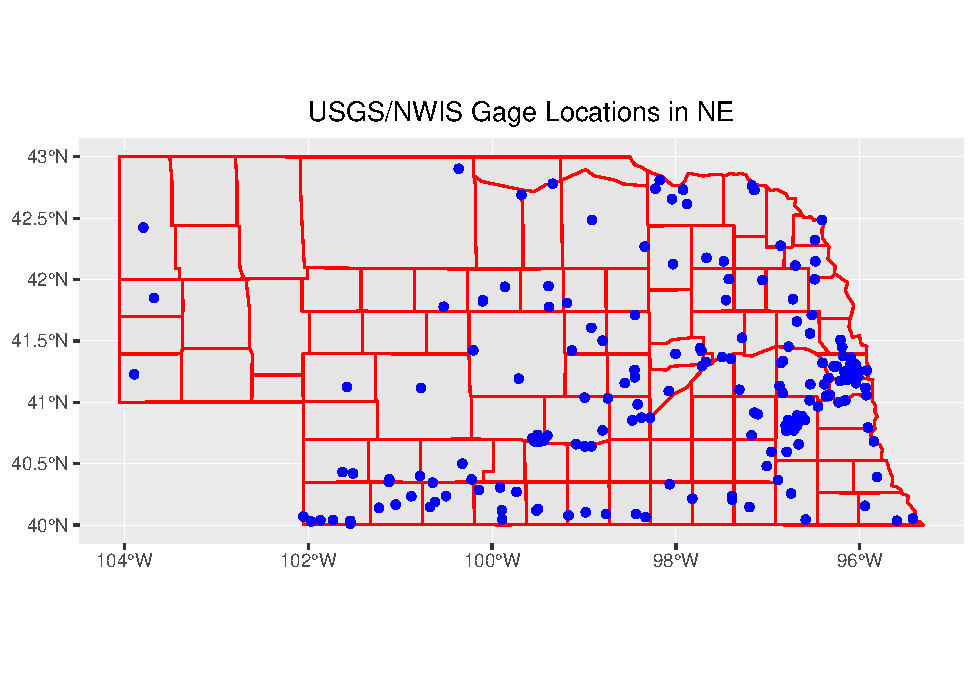
\includegraphics{A06_GLMs_files/figure-latex/unnamed-chunk-2-1.pdf}

\begin{Shaded}
\begin{Highlighting}[]
\CommentTok{#5}

\KeywordTok{bartlett.test}\NormalTok{(Neonicotinoids.Raw}\OperatorTok{$}\NormalTok{Pub..Year }\OperatorTok{~}\StringTok{ }\NormalTok{Neonicotinoids.Raw}\OperatorTok{$}\NormalTok{Chemical.Name)}
\end{Highlighting}
\end{Shaded}

\begin{verbatim}
## 
##  Bartlett test of homogeneity of variances
## 
## data:  Neonicotinoids.Raw$Pub..Year by Neonicotinoids.Raw$Chemical.Name
## Bartlett's K-squared = 139.59, df = 8, p-value < 2.2e-16
\end{verbatim}

\begin{Shaded}
\begin{Highlighting}[]
\CommentTok{# Test results: K^2 = 139.59, df = 8, p < 0.001}
\CommentTok{# Since p < 0.05, this is evidence that the variance in frequency of years is significantly different for the different chemicals.}
\end{Highlighting}
\end{Shaded}

\begin{enumerate}
\def\labelenumi{\arabic{enumi}.}
\setcounter{enumi}{5}
\tightlist
\item
  Based on your results, which test would you choose to run to answer
  your research question?
\end{enumerate}

\begin{quote}
ANSWER: A one-way anova is appropriate because there is 1 categorical
explanatory variable (chemical) with more than 2 categories (there are 9
chemicals), and a continous response (count of publications).
\end{quote}

\begin{enumerate}
\def\labelenumi{\arabic{enumi}.}
\setcounter{enumi}{6}
\item
  Run this test below.
\item
  Generate a boxplot representing the range of publication years for
  each chemical. Adjust your graph to make it pretty.
\end{enumerate}

\begin{Shaded}
\begin{Highlighting}[]
\CommentTok{#7}

\NormalTok{pub.year.anova <-}\StringTok{ }\KeywordTok{lm}\NormalTok{(Neonicotinoids.Raw}\OperatorTok{$}\NormalTok{Pub..Year }\OperatorTok{~}\StringTok{ }\NormalTok{Neonicotinoids.Raw}\OperatorTok{$}\NormalTok{Chemical.Name)}
\KeywordTok{summary}\NormalTok{(pub.year.anova)}
\end{Highlighting}
\end{Shaded}

\begin{verbatim}
## 
## Call:
## lm(formula = Neonicotinoids.Raw$Pub..Year ~ Neonicotinoids.Raw$Chemical.Name)
## 
## Residuals:
##     Min      1Q  Median      3Q     Max 
## -18.366  -3.993   1.889   4.889  13.441 
## 
## Coefficients:
##                                               Estimate Std. Error  t value
## (Intercept)                                  2005.9926     0.6082 3298.222
## Neonicotinoids.Raw$Chemical.NameClothianidin    2.0479     1.0246    1.999
## Neonicotinoids.Raw$Chemical.NameDinotefuran    -3.4333     1.1057   -3.105
## Neonicotinoids.Raw$Chemical.NameImidacloprid    3.1181     0.6651    4.689
## Neonicotinoids.Raw$Chemical.NameImidaclothiz    6.4518     2.4412    2.643
## Neonicotinoids.Raw$Chemical.NameNitenpyram      7.7216     1.6630    4.643
## Neonicotinoids.Raw$Chemical.NameNithiazine    -17.6290     1.6299  -10.816
## Neonicotinoids.Raw$Chemical.NameThiacloprid     1.6394     0.9190    1.784
## Neonicotinoids.Raw$Chemical.NameThiamethoxam    4.3738     0.8261    5.295
##                                              Pr(>|t|)    
## (Intercept)                                   < 2e-16 ***
## Neonicotinoids.Raw$Chemical.NameClothianidin  0.04584 *  
## Neonicotinoids.Raw$Chemical.NameDinotefuran   0.00194 ** 
## Neonicotinoids.Raw$Chemical.NameImidacloprid 3.05e-06 ***
## Neonicotinoids.Raw$Chemical.NameImidaclothiz  0.00832 ** 
## Neonicotinoids.Raw$Chemical.NameNitenpyram   3.78e-06 ***
## Neonicotinoids.Raw$Chemical.NameNithiazine    < 2e-16 ***
## Neonicotinoids.Raw$Chemical.NameThiacloprid   0.07467 .  
## Neonicotinoids.Raw$Chemical.NameThiamethoxam 1.40e-07 ***
## ---
## Signif. codes:  0 '***' 0.001 '**' 0.01 '*' 0.05 '.' 0.1 ' ' 1
## 
## Residual standard error: 7.093 on 1274 degrees of freedom
## Multiple R-squared:  0.1726, Adjusted R-squared:  0.1674 
## F-statistic: 33.21 on 8 and 1274 DF,  p-value: < 2.2e-16
\end{verbatim}

\begin{Shaded}
\begin{Highlighting}[]
\CommentTok{# see the summary table for individual results (t values, p values)}

\CommentTok{#8}

\NormalTok{pub.year.boxplot <-}\StringTok{ }\KeywordTok{ggplot}\NormalTok{(Neonicotinoids.Raw) }\OperatorTok{+}
\StringTok{  }\KeywordTok{geom_boxplot}\NormalTok{(}\KeywordTok{aes}\NormalTok{(}\DataTypeTok{x =}\NormalTok{ Chemical.Name, }\DataTypeTok{y =}\NormalTok{ Pub..Year)) }\OperatorTok{+}
\StringTok{  }\KeywordTok{xlab}\NormalTok{(}\StringTok{"Chemicals"}\NormalTok{) }\OperatorTok{+}
\StringTok{  }\KeywordTok{ylab}\NormalTok{(}\StringTok{"Publication Years"}\NormalTok{) }\OperatorTok{+}\StringTok{ }
\StringTok{  }\KeywordTok{ggtitle}\NormalTok{(}\StringTok{"Publication Years of Neonicotinoid Chemicals"}\NormalTok{) }\OperatorTok{+}\StringTok{ }
\StringTok{  }\KeywordTok{theme}\NormalTok{(}\DataTypeTok{axis.text.x =} \KeywordTok{element_text}\NormalTok{(}\DataTypeTok{angle =} \DecValTok{90}\NormalTok{, }\DataTypeTok{hjust =} \DecValTok{1}\NormalTok{))}
\KeywordTok{print}\NormalTok{(pub.year.boxplot)}
\end{Highlighting}
\end{Shaded}

\includegraphics{A06_GLMs_files/figure-latex/unnamed-chunk-3-1.pdf}

\begin{enumerate}
\def\labelenumi{\arabic{enumi}.}
\setcounter{enumi}{8}
\tightlist
\item
  How would you summarize the conclusion of your analysis? Include a
  sentence summarizing your findings and include the results of your
  test in parentheses at the end of the sentence.
\end{enumerate}

\begin{quote}
ANSWER: Studies on various neonicotinoid chemicals were conducted in
different years - this is concluded by statistically different means of
the publication years of the chemicals. (Using a linear model, residual
standard error: 7.093 on 1274 degrees of freedom, adjusted R-squared:
0.1674, F-statistic: 33.21, p-value: \textless{} 2.2e-16)
\end{quote}

\subsection{NTL-LTER test}\label{ntl-lter-test}

Research question: What is the best set of predictors for lake
temperatures in July across the monitoring period at the North Temperate
Lakes LTER?

\begin{enumerate}
\def\labelenumi{\arabic{enumi}.}
\setcounter{enumi}{10}
\tightlist
\item
  Wrangle your NTL-LTER dataset with a pipe function so that it contains
  only the following criteria:
\end{enumerate}

\begin{itemize}
\tightlist
\item
  Only dates in July (hint: use the daynum column). No need to consider
  leap years.
\item
  Only the columns: lakename, year4, daynum, depth, temperature\_C
\item
  Only complete cases (i.e., remove NAs)
\end{itemize}

\begin{enumerate}
\def\labelenumi{\arabic{enumi}.}
\setcounter{enumi}{11}
\tightlist
\item
  Run an AIC to determine what set of explanatory variables (year4,
  daynum, depth) is best suited to predict temperature. Run a multiple
  regression on the recommended set of variables.
\end{enumerate}

\begin{Shaded}
\begin{Highlighting}[]
\CommentTok{#11}

\CommentTok{# July is daynum 182-212}

\NormalTok{NTL.ChemPhys.processed <-}\StringTok{ }
\StringTok{  }\NormalTok{NTL.ChemPhys }\OperatorTok
\StringTok{  }\KeywordTok{filter}\NormalTok{(daynum }\OperatorTok{>}\StringTok{ }\DecValTok{181} \OperatorTok{&}\StringTok{ }\NormalTok{daynum }\OperatorTok{<}\StringTok{ }\DecValTok{213}\NormalTok{) }\OperatorTok\StringTok{ }\CommentTok{# take only dates in July}
\StringTok{  }\KeywordTok{select}\NormalTok{(lakename, year4, daynum, depth, temperature_C) }\OperatorTok\StringTok{ }\CommentTok{# choose these columns}
\StringTok{  }\KeywordTok{na.omit}\NormalTok{() }\CommentTok{# remove any row with NA}

\CommentTok{#12}

\CommentTok{# run step AIC}
\NormalTok{NTL.AIC <-}\StringTok{ }\KeywordTok{lm}\NormalTok{(}\DataTypeTok{data =}\NormalTok{ NTL.ChemPhys.processed, temperature_C }\OperatorTok{~}\StringTok{ }\NormalTok{year4 }\OperatorTok{+}\StringTok{ }\NormalTok{daynum }\OperatorTok{+}\StringTok{ }
\StringTok{              }\NormalTok{depth)}
\KeywordTok{step}\NormalTok{(NTL.AIC)}
\end{Highlighting}
\end{Shaded}

\begin{verbatim}
## Start:  AIC=26016.31
## temperature_C ~ year4 + daynum + depth
## 
##          Df Sum of Sq    RSS   AIC
## <none>                141118 26016
## - year4   1        80 141198 26020
## - daynum  1      1333 142450 26106
## - depth   1    403925 545042 39151
\end{verbatim}

\begin{verbatim}
## 
## Call:
## lm(formula = temperature_C ~ year4 + daynum + depth, data = NTL.ChemPhys.processed)
## 
## Coefficients:
## (Intercept)        year4       daynum        depth  
##    -6.45556      0.01013      0.04134     -1.94726
\end{verbatim}

\begin{Shaded}
\begin{Highlighting}[]
\CommentTok{# run multiple regression on recommended model}
\NormalTok{NTL.model <-}\StringTok{ }\KeywordTok{lm}\NormalTok{(}\DataTypeTok{data =}\NormalTok{ NTL.ChemPhys.processed, temperature_C }\OperatorTok{~}\StringTok{ }\NormalTok{year4 }\OperatorTok{+}\StringTok{ }\NormalTok{daynum }\OperatorTok{+}\StringTok{ }\NormalTok{depth)}
\KeywordTok{summary}\NormalTok{(NTL.model)}
\end{Highlighting}
\end{Shaded}

\begin{verbatim}
## 
## Call:
## lm(formula = temperature_C ~ year4 + daynum + depth, data = NTL.ChemPhys.processed)
## 
## Residuals:
##     Min      1Q  Median      3Q     Max 
## -9.6517 -2.9937  0.0855  2.9692 13.6171 
## 
## Coefficients:
##              Estimate Std. Error  t value Pr(>|t|)    
## (Intercept) -6.455560   8.638808   -0.747   0.4549    
## year4        0.010131   0.004303    2.354   0.0186 *  
## daynum       0.041336   0.004315    9.580   <2e-16 ***
## depth       -1.947264   0.011676 -166.782   <2e-16 ***
## ---
## Signif. codes:  0 '***' 0.001 '**' 0.01 '*' 0.05 '.' 0.1 ' ' 1
## 
## Residual standard error: 3.811 on 9718 degrees of freedom
## Multiple R-squared:  0.7417, Adjusted R-squared:  0.7417 
## F-statistic:  9303 on 3 and 9718 DF,  p-value: < 2.2e-16
\end{verbatim}

\begin{enumerate}
\def\labelenumi{\arabic{enumi}.}
\setcounter{enumi}{12}
\tightlist
\item
  What is the final linear equation to predict temperature from your
  multiple regression? How much of the observed variance does this model
  explain?
\end{enumerate}

\begin{quote}
ANSWER:
\end{quote}

Temperature\_C = -6.455560 + 0.010131\emph{year4 + 0.041336}daynum
-1.947264*depth

The adjusted R-squared value shows that 0.7417 of the observed variance
is explained by this model.

\begin{enumerate}
\def\labelenumi{\arabic{enumi}.}
\setcounter{enumi}{13}
\tightlist
\item
  Run an interaction effects ANCOVA to predict temperature based on
  depth and lakename from the same wrangled dataset.
\end{enumerate}

\begin{Shaded}
\begin{Highlighting}[]
\CommentTok{#14}

\NormalTok{NTL.ancova <-}\StringTok{ }\KeywordTok{lm}\NormalTok{(}\DataTypeTok{data =}\NormalTok{ NTL.ChemPhys.processed, temperature_C }\OperatorTok{~}\StringTok{ }\NormalTok{depth }\OperatorTok{*}\StringTok{ }\NormalTok{lakename)}
\KeywordTok{summary}\NormalTok{(NTL.ancova)}
\end{Highlighting}
\end{Shaded}

\begin{verbatim}
## 
## Call:
## lm(formula = temperature_C ~ depth * lakename, data = NTL.ChemPhys.processed)
## 
## Residuals:
##     Min      1Q  Median      3Q     Max 
## -7.6455 -2.9133 -0.2879  2.7567 16.3606 
## 
## Coefficients:
##                                Estimate Std. Error t value Pr(>|t|)    
## (Intercept)                     22.9455     0.5861  39.147  < 2e-16 ***
## depth                           -2.5820     0.2411 -10.711  < 2e-16 ***
## lakenameCrampton Lake            2.2173     0.6804   3.259  0.00112 ** 
## lakenameEast Long Lake          -4.3884     0.6191  -7.089 1.45e-12 ***
## lakenameHummingbird Lake        -2.4126     0.8379  -2.879  0.00399 ** 
## lakenamePaul Lake                0.6105     0.5983   1.020  0.30754    
## lakenamePeter Lake               0.2998     0.5970   0.502  0.61552    
## lakenameTuesday Lake            -2.8932     0.6060  -4.774 1.83e-06 ***
## lakenameWard Lake                2.4180     0.8434   2.867  0.00415 ** 
## lakenameWest Long Lake          -2.4663     0.6168  -3.999 6.42e-05 ***
## depth:lakenameCrampton Lake      0.8058     0.2465   3.268  0.00109 ** 
## depth:lakenameEast Long Lake     0.9465     0.2433   3.891  0.00010 ***
## depth:lakenameHummingbird Lake  -0.6026     0.2919  -2.064  0.03903 *  
## depth:lakenamePaul Lake          0.4022     0.2421   1.662  0.09664 .  
## depth:lakenamePeter Lake         0.5799     0.2418   2.398  0.01649 *  
## depth:lakenameTuesday Lake       0.6605     0.2426   2.723  0.00648 ** 
## depth:lakenameWard Lake         -0.6930     0.2862  -2.421  0.01548 *  
## depth:lakenameWest Long Lake     0.8154     0.2431   3.354  0.00080 ***
## ---
## Signif. codes:  0 '***' 0.001 '**' 0.01 '*' 0.05 '.' 0.1 ' ' 1
## 
## Residual standard error: 3.471 on 9704 degrees of freedom
## Multiple R-squared:  0.7861, Adjusted R-squared:  0.7857 
## F-statistic:  2097 on 17 and 9704 DF,  p-value: < 2.2e-16
\end{verbatim}

\begin{enumerate}
\def\labelenumi{\arabic{enumi}.}
\setcounter{enumi}{14}
\tightlist
\item
  Is there an interaction between depth and lakename? How much variance
  in the temperature observations does this explain?
\end{enumerate}

\begin{quote}
ANSWER: The ancova model shows that there is an interaction between
depth and lakename, as illustrated by the overall p-value \textless{}
2.2e-16. However, some of the p values corresponding to the interactions
between depth and specific lakes are not \textless{} 0.05, which
suggests that this interaction is not significant for all lakes. The
adjusted R-squared value shows that 0.7857 of the observed temperature
variance is explained by this model.
\end{quote}

\begin{enumerate}
\def\labelenumi{\arabic{enumi}.}
\setcounter{enumi}{15}
\tightlist
\item
  Create a graph that depicts temperature by depth, with a separate
  color for each lake. Add a geom\_smooth (method = ``lm'', se = FALSE)
  for each lake. Make your points 50 \% transparent. Adjust your y axis
  limits to go from 0 to 35 degrees. Clean up your graph to make it
  pretty.
\end{enumerate}

\begin{Shaded}
\begin{Highlighting}[]
\CommentTok{#16}

\NormalTok{temp_by_depth <-}\StringTok{ }\KeywordTok{ggplot}\NormalTok{(NTL.ChemPhys.processed, }\KeywordTok{aes}\NormalTok{(}\DataTypeTok{x =}\NormalTok{ depth, }\DataTypeTok{y =}\NormalTok{ temperature_C)) }\OperatorTok{+}
\StringTok{  }\KeywordTok{geom_point}\NormalTok{(}\KeywordTok{aes}\NormalTok{(}\DataTypeTok{color =}\NormalTok{ lakename), }\DataTypeTok{alpha=}\FloatTok{0.5}\NormalTok{, }\DataTypeTok{stroke=}\DecValTok{0}\NormalTok{) }\OperatorTok{+}\StringTok{ }
\StringTok{  }\KeywordTok{geom_smooth}\NormalTok{(}\DataTypeTok{method=}\NormalTok{lm, }\DataTypeTok{se=}\OtherTok{FALSE}\NormalTok{, }\KeywordTok{aes}\NormalTok{(}\DataTypeTok{color =}\NormalTok{ lakename)) }\OperatorTok{+}\StringTok{ }\CommentTok{# add line of best fit for each lake}
\StringTok{  }\KeywordTok{ylim}\NormalTok{(}\DecValTok{0}\NormalTok{, }\DecValTok{35}\NormalTok{) }\OperatorTok{+}\StringTok{ }\CommentTok{# zoom into concentration of points}
\StringTok{  }\KeywordTok{ggtitle}\NormalTok{(}\StringTok{"Temperature vs Depth, by Lake"}\NormalTok{) }\OperatorTok{+}\StringTok{ }\CommentTok{# add main title}
\StringTok{  }\KeywordTok{xlab}\NormalTok{(}\StringTok{"Depth (m)"}\NormalTok{) }\OperatorTok{+}\StringTok{ }\CommentTok{# format labels with UOM}
\StringTok{  }\KeywordTok{ylab}\NormalTok{(}\StringTok{"Temperature (C)"}\NormalTok{)}
\KeywordTok{print}\NormalTok{(temp_by_depth)}
\end{Highlighting}
\end{Shaded}

\begin{verbatim}
## Warning: Removed 73 rows containing missing values (geom_smooth).
\end{verbatim}

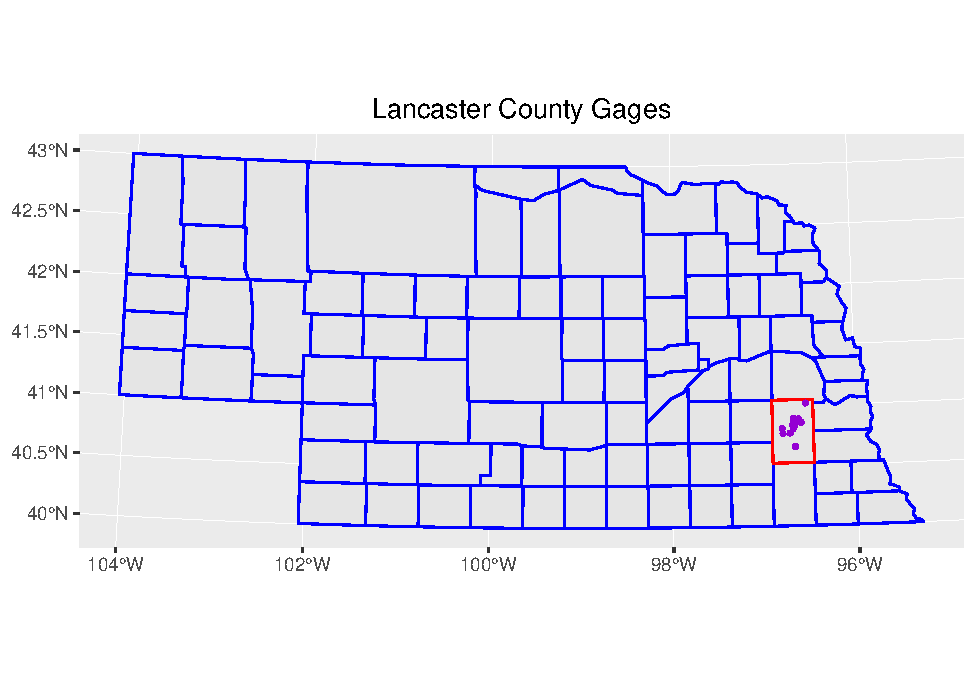
\includegraphics{A06_GLMs_files/figure-latex/unnamed-chunk-6-1.pdf}


\end{document}
